\chapter{Kod odcisku}

Rozdział ten poświęcony jest opisowi zastosowanego algorytmu, pozwalającego na uzyskanie kodu odcisku.
Metody opisywane w poprzednim rozdziale skupiają się na porównywaniu obiektów(minucji) uwzględniając ich położenie, kąt oraz typ. 
Zaawansowane algorytmy wykorzystują dodatkowo jakość odcisku (jest to wyliczana dla każdej minucji wielkość na podstawie 
jakości próbki biometrycznej). Kolejną cechą którą można brać pod uwagę jest wzajemna korelacja minucji. Dopasowane minucje
można utożsamiać z wierzchołkami grafu, wtedy dopasowywane punkty w obu obrazach powinny być podobne. 

Wadą takiego podejścia jest ich złożoność obliczeniowa dlatego zaproponowano podejście prostsze, opierające się 
na stworzeniu kodu odcisku. Dodatkowo aktualne rozwiązania stwierdzają zgodność w porównywaniu odcisków biorąc pod uwagę ilość zgodnych minucji.
Kod odcisku umożliwia porównywanie całości próbki biometrycznej nie tylko jej części podobnej.

\section[Algorytm Kodujący][Algorytm Kodujący]{Algorytm Kodujący}

Tworzony algorytm od samego początku miał narzucone ograniczenia a mianowicie:
\renewcommand*{\labelitemi}{\bullet}
\begin{itemize}
\item unikanie podejścia obiektowego
\item możliwie jak najprostszy 
\item łatwo konfigurowalny
\item prosta funkcja porównująca kody(najlepiej XOR\footnote{ang. {\em Exclusive or} - Alternatywa wykluczająca zwracająca prawdę dla dwóch przeciwnych wartości} )
\item powinien być skuteczny
\item niska złożoność obliczeniowa
\end{itemize}
\vspace{.5cm}\par

O ile spełnienie pierwszych trzech wymagań jest w miarę proste kolejne stwarzają problemy. Prosty algorytm kodujący niekoniecznie będzie miał prostą funkcją porównującą, dodatkowo nie zawsze musi być 
skuteczny. Zwiększanie stopnia skomplikowania algorytmu może skutecznie wpłynąć na jego skuteczność ale zwiększa złożoność obliczeniową. Dodatkowo w trakcie zwiększania trudności algorytmu kod magazynuję
coraz więcej informacji o obrazie stając się niejako innym zapisem metod obiektowych. Nie trudno zauważyć iż spełnienie wszystkich wymagań staję się niemożliwe, a zaproponowane rozwiązanie jest jedynie
najbardziej optymalnym wyjściem z sytuacji

\subsection[Algorytm Kodujący][Naiwny kod]{Naiwny kod} 
Algorytm opiera się na bardzo prostym pojmowaniu kodu odcisku. Algorytm jako wejście otrzymuje listę minucji wraz z ich współrzędnymi XY obrazu oraz kąt minucji. Algorytm zakłada, iż odciski pochodzące od tej samej 
osoby będą miały minucje poukładane w taki sam sposób. Dlatego koduje on sposób ułożenia minucji na odcisku. Zasada działania polega na podziale całego obszaru obrazu na mniejsze fragmenty. Ich wielkość 
jest tak dobrana aby znaczna część minucji znajdowała się samodzielnie w swoich fragmentach. W praktyce zdarza się, że dwie minucje leżą w tym samym fragmencie. 
Ponieważ kształt musi być taki sam dla wszystkich kodów przyjęto iż obszar obrazu podzielony będzie na jednakowe kwadraty tworząc siatkę na obrazie. Kwadrat, w którym znajduje się przynajmniej
jedna minucja oznaczany jest jako "1" w kodzie pozostałe obszary to "0". 
\begin{figure}[hbt]
    \begin{center}
	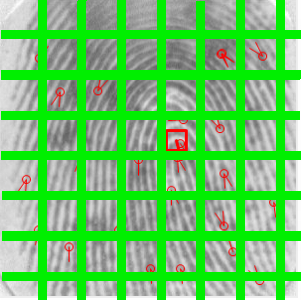
\includegraphics[angle=0,scale=1]{img/fingerprint_with_crate.jpg}
	\caption{Przykładowa siatka kodowa na tle odcisku}
	\label{simple_finger_crate_code}
    \end{center}
\end{figure}
\newline
Na ilustracji \ref{simple_finger_crate_code} można zauważyć fragmenty "kratki w której zmieściły się dwie minucję", po otrzymaniu kodu informacja ta zostanie stracona i silnik porównujący nie będzie 
wiedział czy w kratce była jedna czy więcej minucji. Rzeczywiste porównanie uwzględnia wartości kątów minucji leżących w tym samym kwadracie i dopiero na jej podstawie stwierdza zgodność.

\begin{figure}[hbt]
    \begin{center}
	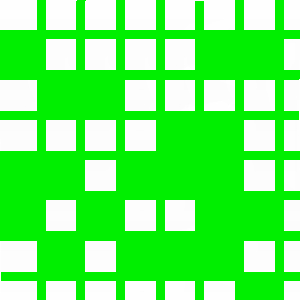
\includegraphics[angle=0,scale=1]{img/simple_crate_code.jpg}
	\caption{Otrzymany kod}
	\label{simple_code}
    \end{center}
\end{figure}
Na rysunku \ref{simple_code} pokazano otrzymany kod, który dla odpowiedniej(stałej) kolejności odczytywania utworzy binarny kod zer i jedynek.

\subsubsection{Ocena przydatności}
\begin{enumerate}
\item Zalety rozwiązania
\renewcommand*{\labelitemi}{\bullet}
\begin{itemize}
\item prostota algorytmu
\item kod odcisku zajmuje bardzo mało pamięci
\item XOR jako funkcja porównująca kody
\item bardzo niska złożoność obliczeniowa
\end{itemize}
\item Wady rozwiązania
\renewcommand*{\labelitemi}{\bullet}
\begin{itemize}
\item utrata informacji o minucji w przypadku za dużych podprzestrzeni
\item wrażliwość na przekształcenia
\item niska, wręcz zerowa skuteczność porównywania odcisków
\item wysoka wrażliwość na odciski o bardzo dużej liczbie minucji
\end{itemize}
\end{enumerate}

\vspace{.5cm}\par

Reasumując rozwiązanie tego typu nie można w żadnym stopni nazywać biometrią, zastosowane zostało jedynie jako wprawka dla następnych wersji algorytmu kodującego.
Ponieważ algorytm jest nieskuteczny należy zastanowić się nad przyczynami jego wad. Po pierwsze utratę informacji o minucjach zlokalizowanych w tej samej podprzestrzeni można zniwelować poprzez dodanie 
jeszcze jednego wymiaru do kodu, kąta pomiędzy styczną do grzbietu\footnote{przyjmuje się, że czarne części linii papilarnych nazywane są grzbietami białe dolinami} a osia odciętych. Oczywiście może zdarzyć się, że
minucje początkowo znajdujące się w tej samej podprzestrzeni nawet po dodaniu trzeciej współrzędnej dalej będą się w niej znajdować lecz prawdopodobieństwo to jest mniejsze. Świadczyć o tym może fakt iż
nagromadzenia minucji często znajdują się w miejscach gdzie linie papilarne zakręcają, tworząc pętle i wiry. Kąty tych minucji powinny być zupełnie inne. Rozwiązanie to zapobiega również błędnym 
porównaniom odcisków o dużej liczbie minucji. Odciski takie często mają rozkład minucji powodujący "zakodowanie" większości podprzestrzeni. Sytuacja ta jest na tyle uciążliwa, że dla pewnych wielkości siatki
dowolne dwa odciski były zaznaczane jako pochodzące od tej samej osoby. Dodanie kąta jako trzeciej wartości w kodzie nieco rozprasza zakodowanie. Kolejnym problemem jest wysoka wrażliwość na przekształcenia,
rozwiązaniem było zastosowanie sztucznych przekształceń obrazu i kodowanie wszystkich uzyskanych obrazów. Tworzy się w ten sposób wiele kodów dla jednego odcisku. Wszystkie te rozwiązania mają na celu 
polepszenie skuteczności algorytmu.

\subsection[Algorytm Kodujący][Macierz kodów]{Macierz kodów} 
Opisywany poniżej algorytm jest ulepszoną wersja naiwnego kodowania, eliminującą podstawowe wady pierwszego rozwiązania. Algorytm polega na kodowaniu kolejnych transformacji obrazu odcisku. Transformacje polegają na 
wykonaniu translacji obrazu o sprecyzowane wektory, oraz obracanie 
obrazu dla każdej translacji. Nieruchoma pozostaje ramka w której znajduje się wzorcowy obraz. Minucje które po transformacji znajdują się poza ramką są pomijane. Symuluje to uzyskanie odcisku poprzez 
inne przyłożenie palca do czytnika. Dla każdej otrzymanej transformacji obrazu wejściowego tworzony jest naiwny kod. Przykładowa transformacja obrazu pokazana jest na rysunku \ref{angle_shift} Wynikowym 
kodem odcisku jest sklejenie wszystkich otrzymanych kodów i liczba segmentów kodu czyli liczba translacji wykonanych na obrazie. W praktycznym zastosowaniu nie stosuje transformacji obrazu a jedynie listy 
minucji. W przypadku porównywania stosowana jest zasada wzorzec-próbka. Jeden z odcisków traktowany jest jako odcisk o większej jakości niż drugi, dla niego tworzony jest wyłącznie naiwny kod. Ma to 
odzwierciedlenie w pobieraniu próbek biometrycznych z reguły jest tak, że nad procesem pobierania próbki czuwa osoba odpowiedzialna za system,  odcisk powinien być pobrany poprawnie tak aby był jak 
najlepszej jakości. Drugi odcisk pochodzi z systemu nad którym nikt nie czuwa, dla niego tworzona jest macierz kodów. Dokładnie jak w zastosowaniu codziennym użytkownik systemu proszony jest(najczęściej 
przez automat) o przyłożenie palca do skanera w celu pobrania próbki. Nie ma żadnej gwarancji iż poprawnie złoży próbkę. Założenie to odzwierciedla warunki rzeczywiste pozyskiwania odcisków. Następnym 
krokiem jest porównanie odcisku. Algorytm bierze kod wzorca i porównuje ze wszystkimi 
naiwnymi kodami macierzy kodów. 
\par 
Porównując pojedyncze kody możliwe są trzy przypadki porównań
\renewcommand*{\labelitemi}{\bullet}
\begin{itemize}
\item \textbf{1 : 1} dopasowanie, elementy wzorca są zgodne z próbką
\item \textbf{1 : 0} niedopasowanie wzorca, element wzorca nie istnieje w próbce
\item \textbf{0 : 1} niedopasowanie próbki, element próbki nie istnieje we wzorcu
\end{itemize}
\vspace{.5cm}\par
Wybierany jest najlepszy wynik porównania tzn. taki dla którego liczba porównań 1:1 jest największa. Jako wskaźnik stosowano również
minimalizację liczby niedopasowań wzorca i próbki. Niestety dla takich wymagań algorytm wybierał taką transformację dopasowanego obrazu próbki dla której większość minucji znajdowała się poza ramką obrazu, czyli były pomijane.
Ubocznym skutkiem poprawienia wskaźnika było zmniejszanie liczby porównywanych minucji. Zaburza to rzeczywiste porównywanie kodów.
\begin{figure}[h]
    \begin{center}
	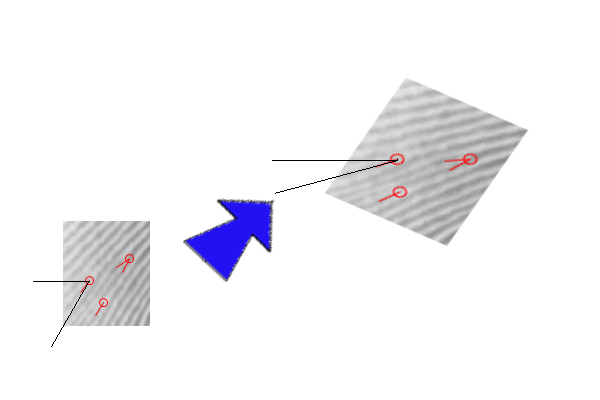
\includegraphics[angle=0,scale=.6]{img/angle_shift.jpg}
	\caption{W trakcie transformacji należy wyliczyć nowe wartości kątów}
	\label{angle_shift}
    \end{center}
\end{figure}

Istotny wpływ na jakość porównania ma wielkość kodu czyli ilość i dokładność informacji w nim przechowywanych. Wielkość kodu musi być dobrana w taki sposób aby dopasowanie było w miarę poprawne i 
jednocześnie ilość obliczeń potrzebnych do porównania nie była zbyt duża. Na wielkość kodu składa się wielkość naiwnego kodu oraz ilość segmentów.

\begin{table}
\begin{tabular}{l l p{13cm}}
\bullet & SC_{size} &  rozmiar naiwnego kodu \\
\bullet & SEG_{size} & ilość segmentów kodowych \\
\bullet & MC_{size} & rozmiar macierzy kodów \\
\bullet & X_{cres} & szerokość (w pikselach) obrazu z odciskiem \\
\bullet & Y_{cres} & wysokość (w pikselach) obrazu z odciskiem \\
\bullet & A_{cres} & zakres kąta(podawany w stopniach) obrazu z odciskiem\\
\bullet & A_{res} & wartość kąta(podawana w stopniach) o jaką maksymalnie należy obracać obraz\\
\bullet & C_{sep} & rozmiar kratki kodu \\
\bullet & X_{step} & odstęp w poziomie pomiędzy najbliższymi translacjami obrazu \\
\bullet & Y_{step} & odstęp w pionie pomiędzy najbliższymi translacjami obrazu \\
\bullet & COV_{step} & wskaźnik odstępu pomiędzy najbliższymi translacjami podawany jako wielokrotność kratki kodu \\
\bullet & A_{step} & odstęp kątowy pomiędzy najbliższymi obrotami obrazu\\
\end{tabular}
\end{table}

\begin{equation}
SC_{size}=[ \frac{X_{cres}}{C_{sep}}] * [ \frac{Y_{cres}}{C_{sep}}]* [ \frac{A_{cres}}{A_{sep}}]\qedhere \\
\label{eq:SC_size}
\end{equation}

\begin{equation}
X_{step}=[ X_{cres} * COV_{step}]
\label{eq:x_step}
\end{equation}

\begin{equation}
Y_{step}=[ Y_{cres} * COV_{step}]
\label{eq:y_step}
\end{equation}

\begin{equation}
SEG_{size}=[ \frac{X_{cres}}{X_{step}}] * [ \frac{Y_{cres}}{Y_{step}}] * [2*\frac{A_{res}}{A_{step}}] \qedhere \\
\label{eq:SEG_size}
\end{equation}

\begin{equation}
MC_{size}=SEG_{size}*SC_{size} \qedhere \\
\label{eq:MC_size}
\end{equation}

\subsubsection{Przykład 1}
Dla obrazu o wymiarach [300 x 300 x 300], rozmiarze kratki kodu [25 x 25 x 30], wskaźniku odstępu 0.5 i odstępie kątowym 15$^\circ$ i maksymalnym kącie obroty 45$^\circ$ otrzymano kod o 
2500 segmentów o wielkości jednego segmentu 1440 bitów(0,175kB) co daje razem 3600000 bitów(0,429Mb). 

\subsubsection{Ocena przydatności}

\begin{enumerate}
\item Zalety rozwiązania
\renewcommand*{\labelitemi}{\bullet}
\begin{itemize}
\item prostoty algorytm kodujący
\item eliminuje podstawowe wady naiwnego kodu
\item skuteczniejszy niż naiwny kod
\item łatwość konfiguracji
\end{itemize}
\item Wady rozwiązania
\renewcommand*{\labelitemi}{\bullet}
\begin{itemize}
\item utrata informacji o minucji w przypadku za dużych podprzestrzeni
\item wrażliwość na przekształcenia nieliniowe
\item średnia skuteczność porównywania odcisków
\item duży rozmiar kodu ( większy niż $2^{21}$ mniejszy niż $2^{22}$)
\item brak trywialnej funkcji porównującej kody
\end{itemize}
\end{enumerate}
\vspace{.5cm}\par

Mimo, iż kolejna wersja algorytmu jest lepsza od poprzedniej wciąż nie jest pozbawiona wad. Podobnie jak w poprzednim rozwiązaniu za duży rozmiar kratki kodowej może zniekształcać informacje i prowadzić do 
zbytniego uproszczenia kodu. Duża kratka może obejmować więcej niż jedną minucje. Z drugiej strony zbyt mały rozmiar kratka może prowadzić do zmniejszenia skuteczności algorytmu. Reprezentacja minucji jako 
otoczenia w którym się znajduje ma symulować zniekształcenia obrazu powstałe w procesie pobierania próbki biometrycznej. Należy uzyskać kompromis pomiędzy tolerancją na zniekształcenia, a skutecznością 
dopasowania. Prostą zależność pokazują schematyczne wykresy \ref{img:crate_size}. Algorytm nie jest odporny na przekształcenia nieliniowe. W procesie pobierania próbki biometrycznej zniekształcenia takie 
jak spłaszczanie palca nie musi dotyczyć całej jego powierzchni, nie musi też być równomierne. Algorytm stara się kompensować zniekształcenia poprzez wskazywanie jedynie otoczenia w którym znajduje się 
minucja, a nie jej dokładnego położenia. Dlatego tak istotny jest właściwy dobór wielkości kratki kodu. Przekształcenia mające symulować pobranie próbki w inny sposób niż w procesie rejestracji są 
wykonywane na całym obrazie. Nie trudno się domyśleć, iż może istnieć takie zniekształcenie obrazu którego nie będzie dało się dopasować do wzorca poprzez obroty i przesunięcia całego obrazu. rozwiązaniem 
tego problemu byłoby wprowadzenie przekształceń na fragmentach obrazu, zamiast na całości. Wiąże się to ze sporym wzrostem rozmiaru kodu. Rozwiązanie to nie zostało zastosowane. Skuteczność porównywania 
znacząco wzrosła w porównaniu do poprzedniej metody, szczegółowe wyniki przedstawione są w rozdziale 4. Kolejną wadą jest znaczny wzrost rozmiarów kodu. Rozwiązaniem może być analiza wyglądu kodu. Kod 
odcisku można porównać wyglądem do macierzy rzadkich. Składa się głownie z "0", gdzieniegdzie występują "1". Dlatego można zastosować prostą kompresje zapisując jedynie położenie "1" domyślnie pozostałe 
miejsca w kodzie są "0". Jednak w dobie szybko rozwijającej się techniki i ciągłego postępu pamięć dyskowa jest raczej tania i nie powinno się przejmować obszernością zaproponowanego rozwiązania. 
Zwłaszcza, że baza danych dla jednego wzorca przechowuje jedynie naiwny kod, a nie jego macierz kodów, macierze są tworzone jedynie dla próbek i są przechowywane przez pamięć operacyjną w trakcie 
porównywania. 
\subsubsection{Przykład 2\footnote{Wyniki dotyczą danych podanych w przykładzie 1}}
Baza danych 1 mln wzorców zajmuje 171,66 MB. Gdyby zaszła potrzeba przechowywania macierzy kodów zamiast naiwnego kodu baza zajmowałaby 419,09 GB. 
\subsubsection{Przykład 3\footnotemark[\value{footnote}]}
Algorytm stwierdzając podobieństwo porównuje naiwny kod wzorca z macierzą kodów próbki, porównując każdy element wzorca z odpowiadającym elementem próbki w każdym jej segmencie. W trakcie całego procesu 
algorytm wykonuje 3600000 porównań.
\vspace{.5cm}\par
Jak widać duży rozmiar kodu nie wpływa znacząco na zdolność magazynowania go w bazach danych, natomiast istotny jest w procesie porównywania. Wraz ze wzrostem skomplikowania funkcji kodującej wzrósł 
stopień skomplikowania funkcji porównującej kody. Utrudnienie polega na porównywaniu kodu wzorca z każdym segmentem kodu próbki. Porównanie to podobnie jak w początkowej wersji algorytmu może być wykonane 
funkcją XOR. Zmiana polega na tym, że algorytm spośród wszystkich porównań musi wybrać takie dla którego wystąpiło najwięcej dopasowań (1 : 1). Poniżej przedstawiono schematycznie wpływ wielkości kratki kodu na poprawność i łatwość dopasowania kodów.
\begin{figure}[h]
    \begin{center}
	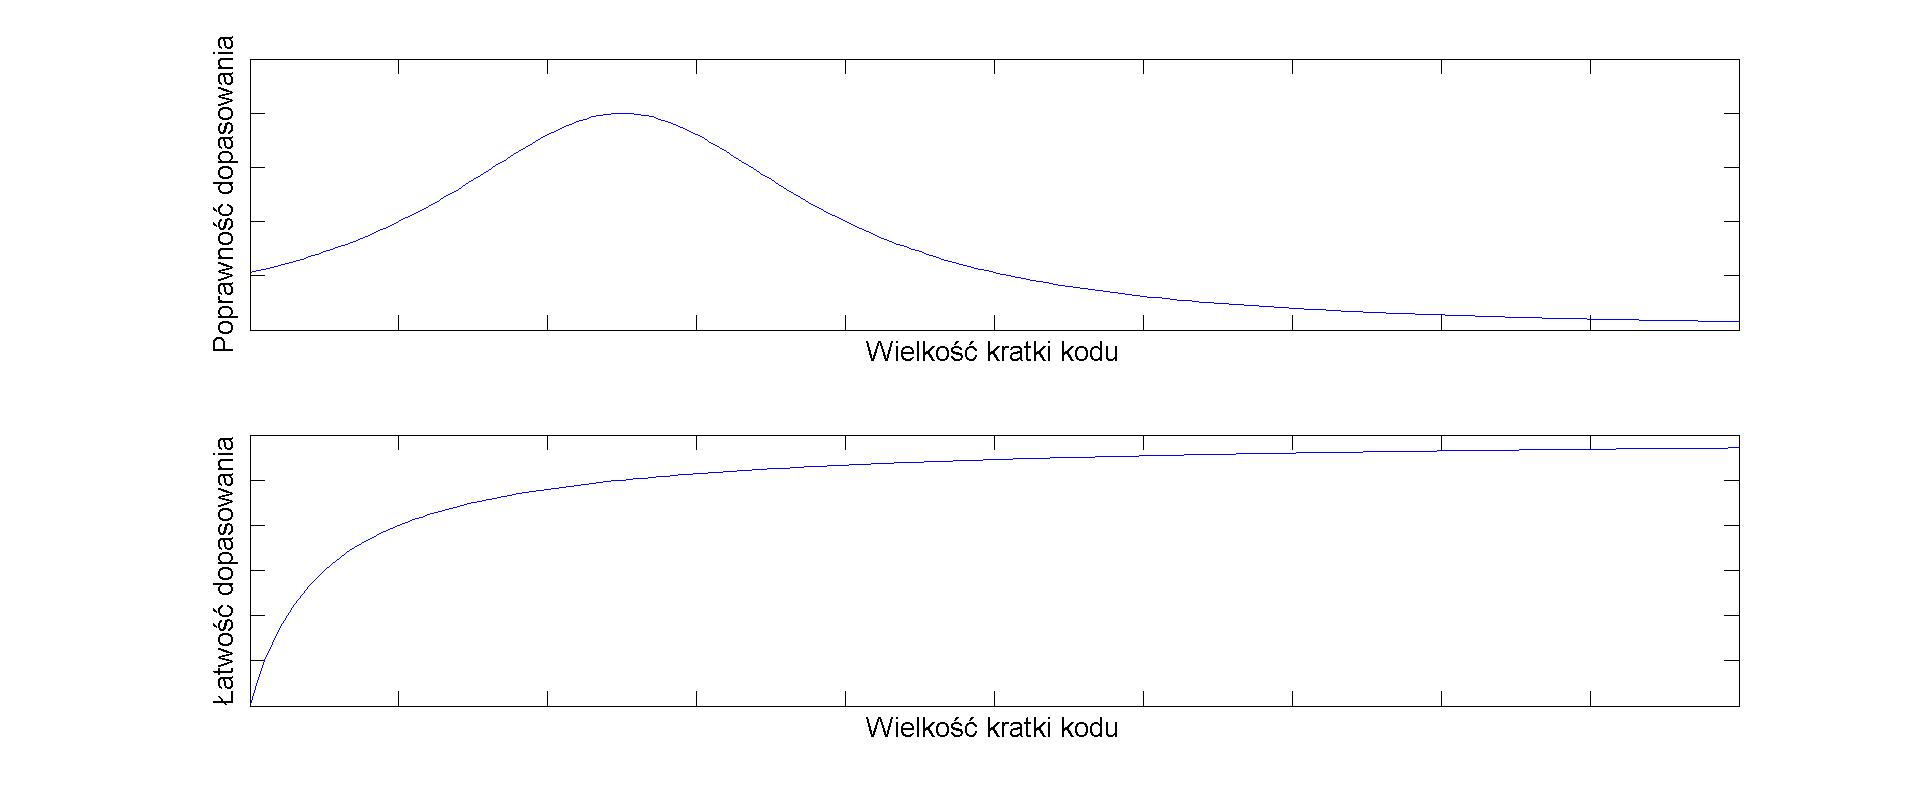
\includegraphics[angle=0,scale=.25]{img/crate_size.jpg}
	\caption{Wpływ wielkości kratki kodu}
	\label{img:crate_size}
    \end{center}
\end{figure}

\section[Przyczyny zastosowań kodu odcisku][Przyczyny zastosowań kodu odcisku]{Przyczyny zastosowań kodu odcisku}

W obecnie istniejących systemach biometrycznych wykorzystujących odcisk palca przeważają metody minucyjne. Jako sposób porównywania obrazów stosowane jest podejście obiektowe. Ideą tej pracy jest 
sprawdzenie możliwości zastosowanie prostego kodowania i odejścia od obiektowego sposobu porównywania odcisków. Praca stara się sprawdzić czy utrwalony model obiektowy o zmiennej liczbie obiektów można 
zastąpić kodem o stałej długości. Weryfikację odcisków można przeprowadzić za pomocą prostej funkcji porównującej. Gdyby rozwiązanie takie wprowadzono w życie, silnik liczący mógłby zostać przeniesiony na 
karty i urządzenia mobilne o ograniczonej mocy obliczeniowej. Weryfikacja mogła by przebiegać bezpośrednio na kartach przenoszonych przez użytkowników. Dodatkowym atutem metody jest pośrednie kodowanie 
informacji biometrycznej. Niepożądane zdobycie kodu odcisku powinno uniemożliwić odtworzenie obrazu lub listy minucji, bez posiadania wiedzy o algorytmie kodującym. Algorytm niekoniecznie musi zapisywać 
położenie minucji w tak prosty sposób jak w przedstawionym powyżej rozwiązaniu. Zawsze możliwe jest dołożenie kilku fałszywych minucji do kodu i zapamietaniu ich położenia. Kolejnym możliwym sposobem 
zabezpieczenia jest odrzucanie wyników zbyt zgodnych. Osoba posiadająca skradziony kod odcisku nie będzie miała możliwości weryfikacji używając skradzionego kodu wzorca. System z łatwością stwierdzi 100\% 
zgodność i z będzie mógł odrzucić próbę fałszerstwa. Dowolne modyfikacje na kodzie w celu wprowadzenia zakłóceń do skradzionego kodu powinno uniemożliwić poprawną weryfikację. Niestety metoda nie jest \
pozbawiona wad. Szczegółowe wyniki działania przedstawiono w rozdziale 4.

